\documentclass[12pt,twoside,slovak,a4paper]{article}

\usepackage[slovak]{babel}
\usepackage[IL2]{fontenc}
\usepackage[utf8]{inputenc}
\usepackage{graphicx}
\usepackage{url}
\usepackage{hyperref}
\usepackage{indentfirst}

\usepackage{cite}

\usepackage[left=2cm, right=2cm, top=3cm, bottom=3cm, bindingoffset=1cm]{geometry}

\pagestyle{headings}

\title{Modelovanie UI pomocou jazyka IFML\thanks{Semestrálny projekt v predmete Metódy inžinierskej práce, ak. rok 2021/22, vedenie: Vladimír Mlynarovic}}

\author{Daniel Belko\\[2pt]
	{\small Slovenská technická univerzita v Bratislave}\\
	{\small Fakulta informatiky a informačných technológií}\\
	{\small \texttt{xbelkod@stuba.sk}}
	}

\date{\small 12. október 2021}

\begin{document}

\maketitle

\begin{abstract}

\end{abstract}



\section{Čo je IFML}

IFML alebo Interactive Flow Modeling Language je vizuálny modelovací jazyk určený pre návrh UI a UX mobilných a webových aplikácii. Cieľom IFML je založiť štandard pre navrhovanie používateľského rozhrania aplikácie a logiku daného rozhrania. Veľkou inspiráciou pre syntax IFML bol modelovací WebML z ktorého bol prebratý koncept kontajnerizácie jednotlivých vrstiev aplikácie a niektoré ďalšie prvky. Výhodou IFML je že jeho prvky sú veľmi všeobecné, čo znamená že sa da využiť na vývoj UI/UX nezávisle od koncovej platformy aplikácie.\cite{BF:IFML}

\section{Čo dokáže IFML}

Keďže IFML má zjednodušené a všeobecné prvky, to znamená že aj modely budú tak isto všeobecné. Čo modely obmedzuje na jednoduché javy, a prechod z jedného kontajnera na ďalší (príklady tohto správania budú neskôr v článku ukázane). To znamená aj že sa pomocou IFML nedá spraviť model komplexných javov, ako napríklad: reťazce operácii.

\clearpage

\section{Jednotlivé prvky IMFL}

\begin{enumerate}
	\item \textbf{Cointainer}
	\begin{itemize}
		\item Prvok ktorý kategorizuje ostatne prvky, môže obsahovať aj ďalšie kontajnery. Napr.: web stránka.
	\end{itemize}
	\item \textbf{View component}
	\begin{itemize}
		\item Vizuálny prvok ktorý niečo ukazuje alebo prijíma vstup. Napr.: Listina kontaktov alebo pole vyhľadávania v prehliadači.
	\end{itemize}
	\item \textbf{Event}
	\begin{itemize}
		\item Jav ktorý zmení stav aplikácie. Napr.: Používateľ klikol na obrázok v galérii a aplikácia priblíži na obrázok.
	\end{itemize}
	\item \textbf{Action}
	\begin{itemize}
		\item Jav ktorý nevykoná UI ale aplikačná logika. Napr.: Odoslanie mailu.
	\end{itemize}
	\item \textbf{Navigation flow}
	\begin{itemize}
		\item Ukazuje z ktorého kontajnera sa vieme dostáť kam a cez aký jav.
	\end{itemize}
	\item \textbf{Data flow}
	\begin{itemize}
		\item Ukazuje do ktorého prvku smerujú údaje.
	\end{itemize}
	\item \textbf{Parameter binding group}
	\begin{itemize}
		\item Zoskupí dôležité parametre (metadata) jednotlivých údajov.
	\end{itemize}
\end{enumerate}

\clearpage

\section{Ukážkový model IFML}

\subsection{Model}

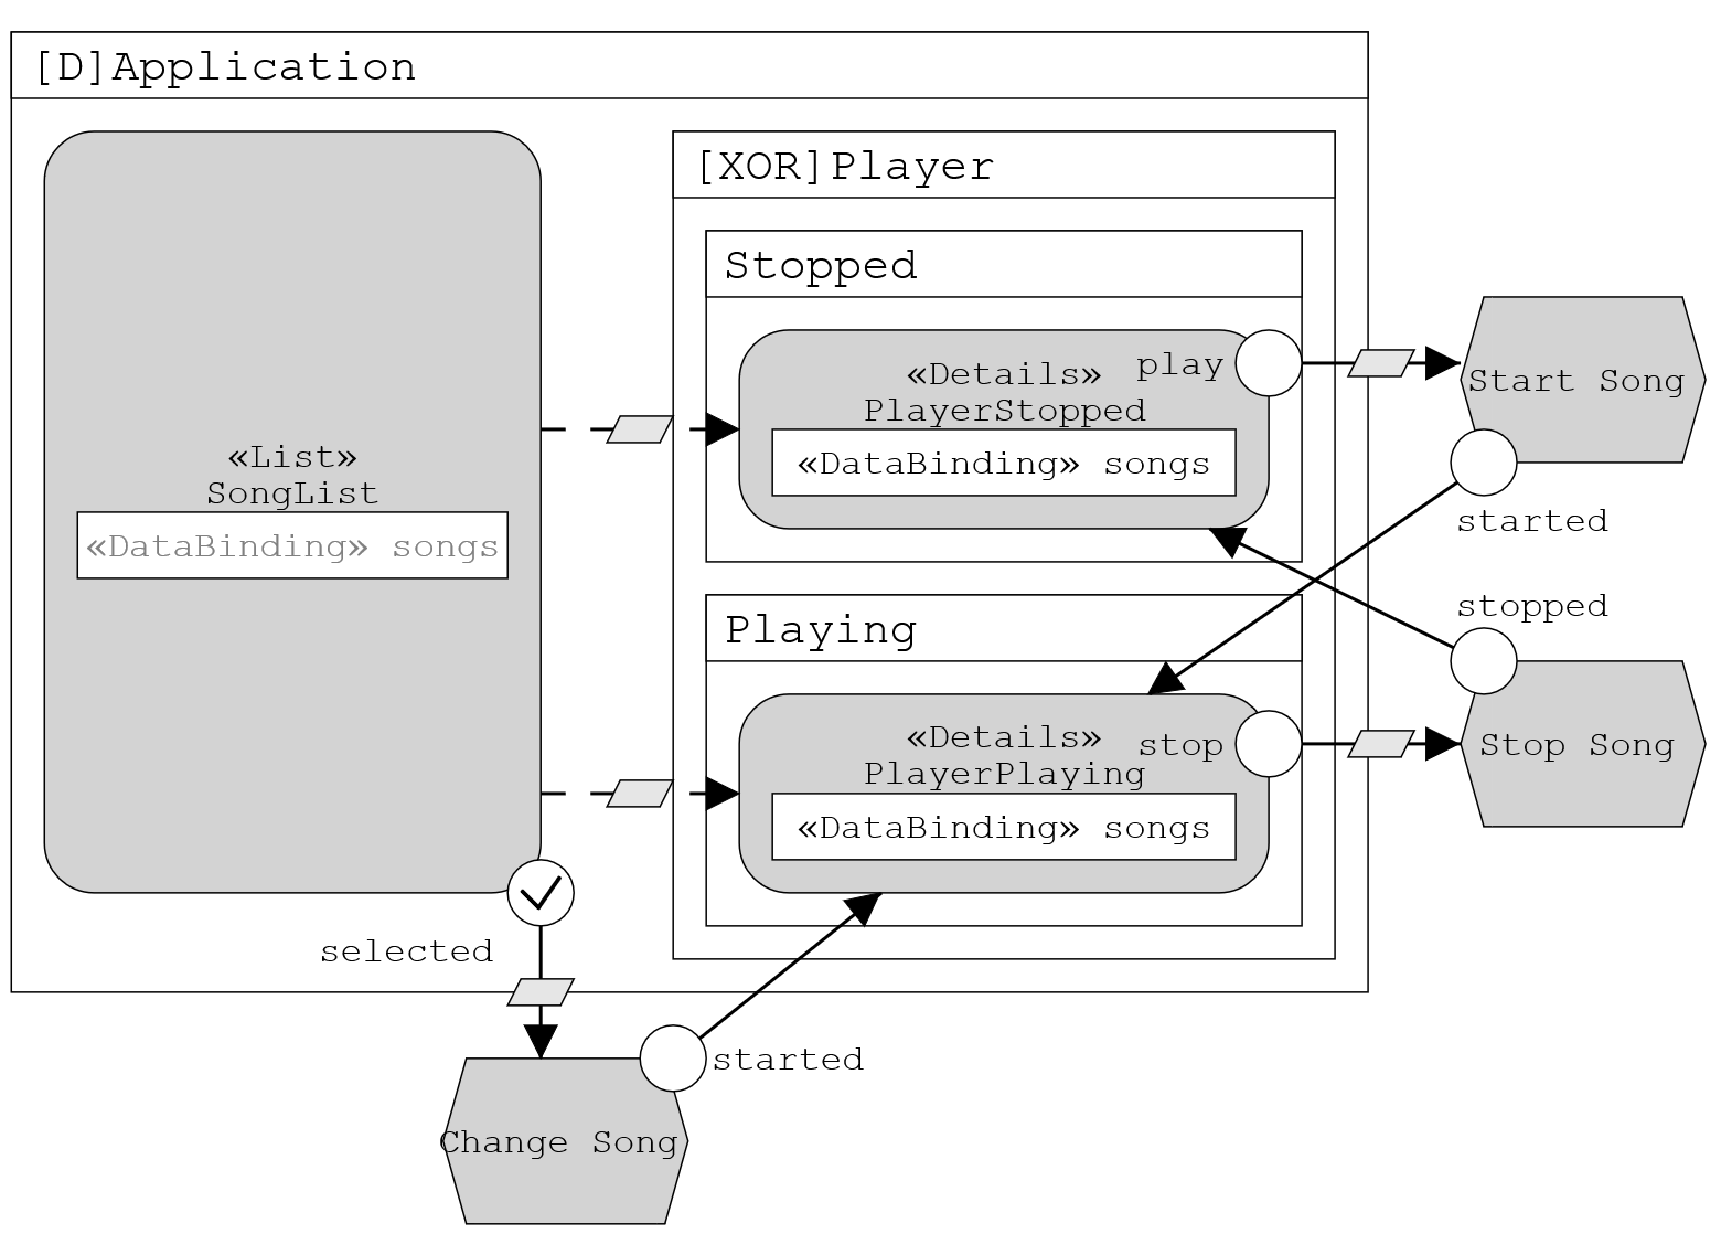
\includegraphics[scale=0.585]{model.pdf}

\subsection{Vysvetlenie}

\bibliography{literatura}
\bibliographystyle{alpha}
\end{document}